% !TEX root = ../main.tex
\section{Illustrative results}
\label{sec:results}

Table~\ref{tab:counts} reports all counts used in the example. Treatment A reaches
the target verdict in 12 of 40 assigned trials (30.0\%); treatment B reaches it
in 18 of 40 (45.0\%). Applying Equation~\eqref{eq:contrast} gives a descriptive
difference of 15.0 percentage points. Infrastructure failures account for
2 of 40 trials in A and 1 of 40 in B, respectively. The reported rates retain
these failures in their denominators.

\begin{table}[htbp]
  \caption{Fictional trial counts. Infrastructure failures are included as
  unsuccessful assigned trials and reported separately. These values do not
  describe an executed experiment.}
  \label{tab:counts}
  \centering
  \begin{tabular}{lrrrr}
    \toprule
    Treatment & Assigned trials & Target verdicts & Rate (\%) & Failures \\
    \midrule
    A & 40 & 12 & 30.0 & 2 \\
    B & 40 & 18 & 45.0 & 1 \\
    \bottomrule
  \end{tabular}
\end{table}

Figure~\ref{fig:rates} presents the same rates with marginal uncertainty under
the illustrative binomial model. Marker shapes distinguish the treatments as
well as color. The display communicates the magnitude of the descriptive
comparison while keeping the uncertainty and raw denominators visible.

\begin{figure}[htbp]
  \centering
  % Keep the generated physical width so its 8--9 pt labels stay readable.
  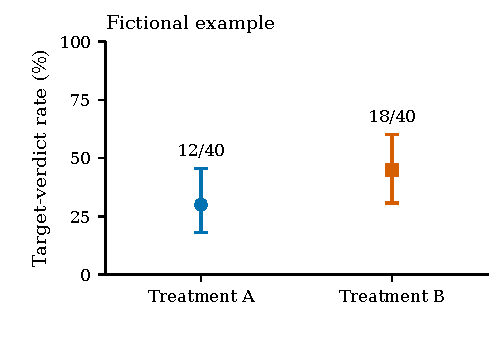
\includegraphics[width=3.35in]{figure-example.pdf}
  \caption{Fictional assigned-trial target-verdict rates. Points show 12/40
  and 18/40 trials, including 2 and 1 infrastructure failures as unsuccessful
  trials. Whiskers show 95\% Wilson score intervals under the independent
  binomial-trial model described in Section~\ref{sec:methods}. No backend,
  model, or experimental treatment was executed to generate these values.}
  \label{fig:rates}
\end{figure}
